\documentclass[12pt,info]{asg}
% General info for the asg.cls file to load
\Instructor{Anna Koop}
\Campus{University of Alberta, Augustana}
\Email{akoop@ualberta.ca}
\Office{Heather Brae 1-31}
\Class{AUCSC 460}
\ClassTitle{Artificial Intelligence}
\Term{Winter 2016}
\Department{Department of Science}


\AsgNum{}
\AsgTitle{Rock-Paper-Scissors Agent Report}
\Due{11:55pm, April 23, 2016}
\Total{25}

\title{Final Project Report}

\begin{document}

\maketitle

Having implemented a rock-paper-scissors agent and tested it against the provided agents, you must now report on what you have done! Your report describes what you did, why you did it that way, and how well it worked. 

\section{Game Agent}
You will be submitting your agent so your instructor can run it against the others.  In {\em addition} to the code, you must provide a written explanation of how it works. Relate to course concepts as necessary. What made you choose the method you did?

\section{Results}
Report empirical results on how it performs. Play matches against the provided agents and report the number of wins. Graphs work best. If your agent program has any tune-able parameters, you should test out different values.

\section{Performance Discussion}
Discuss how it performs. Include any limitations or strengths of your approach. Note that this is separate from the presentation of the results. This is where you examine and explain what the empirical data tells you about the problem and your solution method. Sometimes the results raise more questions than they answer---that's fine, this is where you explicitly raise those questions.

\section{Other Approaches}
Here is where you can demonstrate your understanding of our course content. You don't have to implement other agents, but do describe how you might build a rock-paper-scissors agent in different ways. 

You can think about how you might have implemented an agent for each of our units:
\begin{itemize}
\item Logic-based systems
\item Search
\item Probabilistic Reasoning
\item Supervised Learning
\item Reinforcement Learning
\end{itemize}

\section{Conclusion}
What have you learned about artificial agents as a result of creating this one? Can you draw any conclusions about AI game agents? About the general usefulness of the particular approach you tried?
%%%%%%%%%%%%
%\begin{figure}[bt]
%\label{fig:adder}
%\centering
%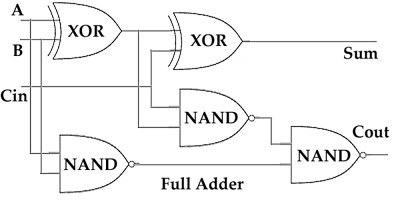
\includegraphics[width=.6\textwidth]{full_adder.png}
%\caption{A (claimed) full-adder circuit}
%\end{figure}

%\newcounter{rubricCat}
%\newcounter{rubricVal}
%\newlength{\colwidth}

%\newenvironment{rubric}[1]{%
%	\setcounter{GradeCategories}{#1}
%	\begin{landscape}
%	\begin{table}[t]
%	\begin{center}
%	\begin{tabulary}{.8\textwidth}{ l | *{5}{c}}
%	 & Excellent & Good & Acceptable & Needs Work & Absentee \\
%	 \end{tabulary}
%	 \end{center}
%	 \end{table}
%	\end{landscape}
%} % rubric environment

\end{document}
